% UTF-8

% single-chapter commands
\documentclass[../main/thesis.tex]{subfiles}
\onlyinsubfile{\setcounter{chapter}{2}}  % single-chapter command
\begin{document}


\chapter{Spezifikation der zu untersuchenden Fälle}

% Plural oder Singular?
% (vgl. Themenblatt)


\section{Vergleich verschiedener Problemfälle der automatisierten Linien-Generalisierung}
\label{ch:case-comparison}

% (Vergleich unter dem Gesichtspunkt der Eignung als „Spezialfall“ für diese DA, vgl. Themenblatt)
% evtl. jeweils ein (Ab)satz zu "worum genau geht es bei diesem Problem" (was nur teilweise offensichtlich ist) und ein (Ab)satz zur Eignung

An dieser Stelle werden zunächst unterschiedliche Spezialfälle beschrieben, in denen die automatisierte Identifikation und Zusammenfassung parallel verlaufender Linienzüge hilfreich wäre.
Der darauf folgende Abschnitt begründet die Auswahl der entsprechend der Aufgabenstellung im Rahmen dieser Arbeit im Weiteren zu behandelnden Spezialfälle.


\subsection{Mehrgleisige Eisenbahnstrecken}

Das Problem der Auswertung der Gleisanzahl mehrgleisiger Bahnstrecken ist bereits in Abschnitt~\ref{railway-case} beschrieben.
Neben der Erkennung solcher Gleise als parallel kann die geometrische Ermittlung der Bahnachse hilfreich für eine ansprechende Visualisierung sein.
Lagepläne im Eisenbahnwesen zeigen sie zusätzlich zu den Gleisachsen, in \osm\ wird sie jedoch nicht erfasst.

% "Bahnachse" https://www-docs.tu-cottbus.de/verkehrswesen/public/Lehre/Lehrbuch/Grundlagen/0-3Zeichnung.pdf


\subsection{Richtungsfahrbahnen im Straßenraum mit baulicher Trennung}
\label{ch:dual-highway-case-desc}

Auch für zweibahnige Straßen, welche in \osm\ als zwei parallele Linienzüge modelliert sind, wird im Gegensatz zum deutschen amtlichen Vermessungswesen \cf[107]{adv08} in \osm\ keine Mittellinie als Achse der Straße erfasst.
Die sich daraus für \osm\ ergebenden Probleme wurden bereits in Abschnitten~\ref{dual-highway-case-1} und~\ref{dual-highway-case-2} beschrieben.
Konkrete Beispiele für solche Straßen sind Autobahnen, aber auch zweibahnige innerstädtische oder Überlandstraßen.

% ATKIS-Objektartenkatalog Basis-DLM 6 (2008)
% http://www.geodatenzentrum.de/docpdf/ATKIS-OK%20Basis-DLM%206_0.pdf


\subsection{Parallele Wege für unterschiedliche Arten von Verkehr}
\label{ch:different-traffic-types-case-desc}

Ein oft zu beobachtendes Muster sind zusammengehörende, jedoch baulich getrennte und damit jeweils als eigene Linienzüge modellierte Verkehrswege für unterschiedliche Fahrzeugtypen, Geschwindigkeitsbereiche oder Zwecke des Verkehrs.
Im Straßenraum zählen dazu:

\begin{itemize}
	\item straßenbegleitende Fuß- und Radwege,
	\item Nebenfahrbahnen \term{(frontage roads)} für Anliegerverkehr, von dem die Hauptfahrbahn freigehalten werden soll,
	% Beispiele: Autobahnen, Kaiserstraße
	\item langgezogene Rampen an teilplanfreien Anschlussstellen insbesondere der Bauformen Diamant und \term{SPUI,}
	% https://de.wikipedia.org/wiki/Anschlussstelle_(Autobahn)
	\item Verteilerfahrbahnen an Doppelanschlussstellen und Autobahnkreuzen,
	% https://de.wikipedia.org/wiki/Autobahnkreuz#Bauteile
	% https://de.wikipedia.org/wiki/Doppelanschlussstelle
	\item Sonderfahrbahnen für Busse, Fahrgemeinschaften oder Mautzahler,
	% https://de.wikipedia.org/wiki/High-occupancy_vehicle_lane#Ausf.C3.BChrung
	\item straßenbündige oder -parallele Bahnkörper,
	\item die Kombination mehrerer der genannten Punkte, etwa als Teil einer komplexen innerstädtischen Straße mit parallelen getrennten Radwegen, Gehwegen, Richtungsfahrbahnen, Nebenfahrbahnen und besonderem Stadtbahn-Gleiskörper.
\end{itemize}

Die sich in solchen Fällen ergebenden Probleme sind vergleichbar zu Abschnitt~\ref{ch:dual-highway-case-desc}, jedoch komplexer, weil die beteiligten Verkehrsarten jeweils unterschiedliche Voraussetzungen haben.
So sind z.~B. straßenbegleitende Radwege aufgrund der geringeren gefahrenen Geschwindigkeiten oft kurviger als die Fahrbahn für Kraftfahrzeuge, sollten aber dennoch als parallel zu ihr gelten können.
Auch erfordern die Unterschiede in Kombination mit Platzmangel oft individuelle bauliche Lösungen, was die Automatisierung der Verarbeitung der Geodaten nicht vereinfacht.


\subsection{Grenzen}

Bisher noch nicht erwähnt wurden unsichtbare Grenzen, deren Verlauf dem physischer Objekte folgt oder zu ihnen parallel ist.
Beispielhaft zu nennen wären Postleitzahlgebiete, deren Grenze einem Straßenzug folgt, oder administrative Grenzen entlang eines Wasserlaufs.
In diesen Fällen setzt die Kartographie die Grenze vom verlaufsgebenden Objekt ab, damit beide Signaturen klar erkennbar sind (Abbildung~\ref{fig:administrative-borders}).
% sg01 ??
In \osm-Karten ist eine solche Generalisierung bisher noch nicht üblich.
% wie werden die Daten statt dessen umgesetzt?
% Streit, ob Unsichtbares überhaupt in OSM rein soll

\begin{figure}[ht]
  \begin{minipage}[t]{.5\linewidth}
    \centering
    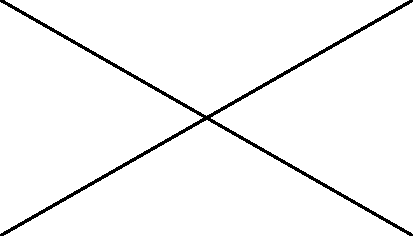
\includegraphics[width=\ScaleIfNeeded]{../image-missing}
    \caption{administrative-borders}\label{fig:administrative-borders}
  \end{minipage}%
  \begin{minipage}[t]{.5\linewidth}
    \centering
    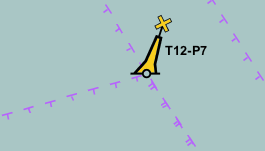
\includegraphics[width=\ScaleIfNeeded]{../chapter3/restricted-area-oseam}
    \caption{restricted-area-oseam}\label{fig:restricted-area-oseam}
  \end{minipage}
\end{figure}

Ein weiteres Beispiel sind zwei aneinander angrenzende Gebiete mit Schifffahrtsbeschränkungen.
Nach den Zeichenregeln für Seekarten ist in solchen Fällen die übliche T-Signatur \cf[B-439.2]{iho13} nur für das gefährlichere der beiden Gebiete zu zeichnen („For coincident limits, the limit symbol (line) portraying the area which is considered to be potentially the most dangerous to navigation [...] has priority.“ \citex[B-439.6~a.]{iho13}).
% S4_4.4.0_EN_Sep13
Eine derartige Abwägung dürfte zwar schon aus rechtlichen Gründen nicht automatisationsfähig sein.
Eine Verbesserung der gegenwärtig unbefriedigenden Darstellung in der auf \osm-Daten basierenden Karte „OpenSeaMap“ (Abbildung~\ref{fig:restricted-area-oseam}) wäre allerdings möglich und anzustreben.

Insgesamt erscheinen Grenzen jedoch im Kontext dieser Arbeit als ein eher schwieriges Feld.
%Während in bestimmten Fällen die üblichen \osm-Karten klare Defizite haben, sind die Fälle, in denen Parallelität eine Rolle spielt, unregelmäßig und 
% Geht das vielleicht schon zu weit?


\subsection{Grundrisstreu erfasste linienhafte Objekte}
\label{ground-plan-linear-objects-case-desc}

Mit zunehmendem Grad der Detaillierung in \osm\ wird versucht, eigentlich linienhafte Objekte als grundrisstreue Fläche zu erfassen.
Für Flüsse ist dies bereits üblich \cf[72]{RT09}, für Straßen und Rollbahnen unter Diskussion.
% http://wiki.openstreetmap.org/w/index.php?title=Key:area&oldid=865108#Highway.2Fpavement_areas
% http://wiki.openstreetmap.org/w/index.php?title=Tag:aeroway%3Drunway&oldid=1218356#How_to_Map
Dadurch entstehen sehr lange und schmale Flächen, deren Ränder größtenteils parallel zueinander sind.
Wenigstens bei Flüssen ist es allerdings etabliert, zusätzlich zur Fläche auch eine Mittellinie in \osm\ zu erfassen.
Daher stellen diese Fälle in der Praxis kein Problem dar und sind für diese Arbeit nicht weiter interessant.


\subsection{Vegetationsgrenzen entlang von Verkehrswegen}

Ein Sonderfall der in Abschnitt~\ref{ground-plan-linear-objects-case-desc} beschriebenen langen und schmalen Flächen sind Waldschneisen.
Im Zuge der immer detaillierteren Erfassung nicht nur des Wegenetzes, sondern auch der Vegetation kommt es vor, dass zusätzlich zu einem durch den Wald führenden Weg auch die sich durch den Weg ergebende Schneise im Wald erfasst wird, indem die Waldfläche in \osm\ in zwei Flächen links und rechts des Wegs aufgeteilt wird (Abbildung~\ref{fig:vegetation-swath-z16}).

Einerseits ermöglicht dies eine präzisere Modellierung der Wirklichkeit, indem die womöglich die Breite des Wegs übersteigende Breite der Schneise modelliert werden kann.
Andererseits werden große Wälder ohnehin gerne in mehrere kleinere Flächen aufgeteilt, um das Arbeiten mit den Geodaten zu vereinfachen.
Schneisen bieten sich dabei als natürliche Stelle zum Aufteilen an.

\begin{figure}[ht]
  \begin{minipage}[t]{.5\linewidth}
    \centering
    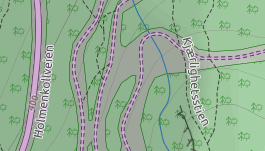
\includegraphics[width=\ScaleIfNeeded]{../chapter3/vegetation-swath-z16}
    \caption{Waldbegrenzung in dieser \osm-Karte dargestellt durch grüne Linie, \term{zoom}~16 (©~Thunderforest)}\label{fig:vegetation-swath-z16}
  \end{minipage}%
  \begin{minipage}[t]{.5\linewidth}
    \centering
    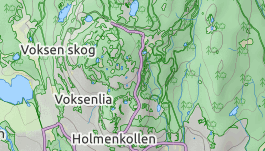
\includegraphics[width=\ScaleIfNeeded]{../chapter3/vegetation-swath-z12}
    \caption{in kleinerem Maßstab Waldschneisen durch grüne Linien unangemessen betont, \term{zoom}~12 (©~Thunderforest)}\label{fig:vegetation-swath-z12}
  \end{minipage}
\end{figure}
% http://www.thunderforest.com/maps/landscape/

Je nach den verwendeten Zeichenregeln werden solche Schneisen in \osm-Karten jedoch stärker betont als wünschenswert (Abbildung~\ref{fig:vegetation-swath-z12}).
Hier wäre eine Erkennung der parallelen Ränder der Schneise hilfreich, um durch Zusammenfassen der Waldfläche das Kartenbild zu verbessern und gleichzeitig zu verhindern, dass durch diese Art der Modellierung entstehende kleinere, von Schneisen umringte Waldparzellen aufgrund von Mindestgrößen automatisch wegfallen.

% allerdings vielleicht hier puffer-methode besser geeignet, schließlich geht es eigentlich um die fläche


%\subsection{Bachläufe und Verkehrswege}
%% das klassische Problem
%
%…





\section{Auswahl der in dieser Arbeit zu behandelnden Spezialfälle}

Viele der bisherigen Arbeiten zur automatisierten Zusammenfassung haben sich mit Straßen beschäftigt (Abschnitt~\ref{ch:existing-approaches}).
In mehreren dieser Arbeiten betonten die Autoren die Wichtigkeit von Ausgangsdaten mit hoher Qualität.
Im Falle von OpenStreetMap ist zu erwarten, dass die Datenqualität für Elemente des Straßennetzes höher ist als die von manch anderen Elementen der \osm-Datenbank.

So gibt es Anhaltspunkte für eine Korrelation zwischen Datenqualität und dem Umstand, ob diese Daten in der Standard-Visualisierung dargestellt werden. \cf[18]{NZZ11}
Dies ist auch anschaulich klar, denn leicht sichtbare Fehler fallen schneller auf und werden somit auch schneller korrigiert als andere Fehler.
Die Standard-Visualisierung der Karte auf \href{https://www.openstreetmap.org/}{\nolinkurl{osm.org}} berücksichtigt viele Details des Straßennetzes.
Unter anderem werden Name und Nummer von Straßen dargestellt, nicht jedoch beispielsweise von Eisenbahnstrecken.
% Highways: Tags für viele Details existieren und werden genutzt. Mehr als für Railways? Vergleich evtl. durch TagInfo möglich, entweder mit historischen Daten (Geofabrik?) oder aber mit aktuellen plus qualitative Überlegung (wann entstand openrailwaymap?)
% TODO: ist der logische Fluss hier ausreichend explizit?

Hinzu kommt die hohe praktische Relevanz des Straßennetzes, die bereits im Namen „OpenStreetMap“ Ausdruck findet, für die \osm-Beitragenden genau wie auch für die Allgemeinbevölkerung.
\osm-Daten werden nicht mehr nur zur visuellen Darstellung, sondern auch zur Navigation verwendet.
Auch dies geht mit einer erhöhten Datenqualität einher. \cf[17–18]{NZZ11}
% Quelle für diesen Punkt nicht großartig; kann dies anhand von Changesets quantifiziert werden?
Verbesserte Algorithmen könnten hier besonders vielen Nutzern zugutekommen.
% TODO: ist der logische Fluss hier ausreichend explizit?

Aus diesen Gründen wird von den zuvor in Abschnitt~\ref{ch:case-comparison} beschriebenen Anwendungsfällen für eine automatisierte Linienzusammenfassung der Fall von \textbf{baulich getrennten Richtungsfahrbahnen im Straßenraum} für diese Arbeit ausgewählt (Abschnitt~\ref{ch:dual-highway-case-desc}).
Solche Straßen sind nahezu allgegenwärtig und die mit deren Darstellung verbundenen Probleme verbreitet.

Die in Abschnitt~\ref{ch:different-traffic-types-case-desc} beschriebenen Fälle paralleler Wege für unterschiedliche Verkehrsarten bieten sich aufgrund ihrer Komplexität nicht an, solange nicht der einfachere Fall von Richtungsfahrbahnen zufriedenstellend gelöst ist.
Es ist jedoch denkbar, dass eine Lösung für bauliche getrennte Richtungsfahrbahnen auch auf einige solcher Fälle übertragbar ist.
Auch auf mehrgleisige Eisenbahnstrecken könnte das Ergebnis dieser Arbeit übertragbar sein.



% single-chapter commands
%\onlyinsubfile{\listoffigures} \onlyinsubfile{\listoftables}
%\onlyinsubfile{% global bibliography settings

\nocite{*}  % include works in bibliography that aren't cited anywhere in the document (for debugging)

\setbibpreamble{Die Literaturangaben sind alphabetisch nach den Nachnamen der Autoren sortiert. Bei mehreren Autoren wird nach dem ersten Autor sortiert.\par\bigskip\bigskip}

\bibliography{../references-papers,../references-manual}
%\bibliography{../references-manual}
}
\end{document}
